% !TeX spellcheck = fr_FR
\chapter{Chapitre 3 : Implémentations}

Dans ce chapitre, on détaillera l'architecture du projet 
ainsi que les technologies et les bibliothèques utilisées
pour développer les différentes parties de l'application.

% L'application produite lors de ce travail de bachelor se base sur une implémentation existante de certains outils réalisés lors d'un projet de semestre.
% Elle est principalement réaliser dans le langage de programmation Rust qui est un langage moderne mutiparadigme, fiable, rapide et sécurisé au niveau de la mémoire.
% Rust utilise des outils dédiés au langage pour accélérer le développement de logiciels dont "cargo" qui est un gestionnaire de paquet et de compilation, "rustdoc", un générateur de documentation à partir du code source et "clippy", un analyseur de code qui indique des erreurs communes réalisées lors de l'écriture du code. 

\section{Rust}

Rust est un langage de programmation système à usage général \footnote{Peut être
utilisé dans l'écriture de kernels ou d'applications}. C'est un langage moderne
et mutiparadigme.
Grâce au principe de \textit{ownership} ou propriété des données, Rust empêche un grand nombre de
bogues lors de l'écriture du code. 
Dans la nomenclature de Rust, le mot "crate" désigne un paquet ou une bibliothèque
externe.
Une particularité de Rust est le \textbf{ownership} ou la propriété des données.

Ce langage permet une compilation vers les plateforme Windows, MacOS et Linux
ainsi que le web grâce au \gls{wasm}. : 

\section{Architecture}

L'application est composée de quatre modules principaux.

\begin{itemize}
	\item Une bibliothèque regroupant des fonctions et des structures communes.
	\item Des utilitaires, ce sont les outils en ligne de commande qui
		implémentes les pipelines 
	\item Un serveur web, celui-ci expose des fichiers pour le client web à
		travers une api \gls{rest}
	\item Un client web permettant à un utilisateur de visualiser des maillages
		dans un navigateur web.
\end{itemize}

En ce qui concerne le module \textit{utilitaire}, l'architecture en pipeline est
utilisé pour tout les binaires. Il est composé de 4 étapes. 
% // TODO: Put pipeline image here

Chacun des utilitaires adapte ce pipeline pour traiter des données spécifique.

\section{Bibliothèque}

La bibliothèque contient les outils de lecture et d'écriture de fichiers pour les formats du chapitre 2.

Elle a comme dépendance principale les crates \textit{stl-io}
qui implémentes les structures pour écrire les fichiers \gls{stl} 
et \textit{las-rs} qui expose les structures et méthodes liées aux données lidar.

\begin{figure}[htbp!]
    \centering
    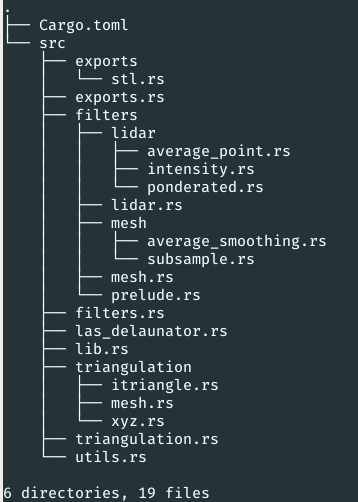
\includegraphics[width=0.5\linewidth]{figures/architecture.png}
    \caption{Structure de fichier présent dans le module de la librairie de l'application. Source : réalisé par Jérôme Chételat}
    \label{fig:library_tree}
\end{figure}

\subsection{Nettoyage}
Les implémentations des filtres sont dérivées du trait \textbf{MeshFilter} ou du trait \textbf{LidarFilter}. Leurs définitions sont les suivantes :
\begin{lstlisting}[language=Rust, style=boxed]
pub trait MeshFilter {
    fn apply(&self, mesh: IndexedMesh, epsilon: f32) -> IndexedMesh;
}

pub trait LidarFilter {
    fn apply(&self, points: Vec<Point>) -> Vec<Point>;
}

\end{lstlisting}

Les traits sont ensuite spécialisés dans le type de filtre voulu.
\subsection{Triangulation}
La librairie contient un module de triangulation.
On y trouve les implémentations des algorithmes de triangulation réalisés lors du projet de semestre, mais également un algorithme de  fusion de triangulation.

\subsection{Fusion de triangulation}
Pour ce qui est de la fusion, une structure propre à la librairie était nécessaire en plus des structures de données offertes par la crates stl-io.
Elle est définie de la manière suivante:
\begin{lstlisting}[language=Rust, style=boxed]
pub struct Mesh {
    /// Vertices composing the mesh
    pub vertices: Vec<XYZ>,
    /// Indexed triangles of the mesh
    pub faces: Vec<usize>,
    /// Indexed vertices part of the convex hull of the mesh
    pub hull: Option<Vec<usize>>,
    /// The neighbourhood of each indexed point
    pub neighbourhood: Option<Vec<HashSet<usize>>>,
}
\end{lstlisting}

La particularité de cette structure est qu'on y trouve un champ pour le voisinage du maillage qui est "neighbourhood" et second champ pour l'enveloppe convexe "hull".
Ils sont optionnels pour maintenir une compatibilité avec les crates utilisées dans la librairie.
Une des raisons vient du fait que lors de la lecture d'un fichier \gls{stl}, on ne retrouve pas ces champs. 

Une méthode utile pour s'assurer de la présence d'un voisinage est d'appeler la fonction neighbourhood.
Elle renvoie le voisinage d'un maillage s'il est déjà présent, le cas échéant est de calculer les voisins.

Son implémentation est disponible dans l'annexe 3. 
Elle parcourt les différents triangles du maillage et pour chaque point présent du triangle, on ajoute ses deux voisins dans une liste.

Cette dernière peut cependant
être améliorée car actuellement, une copie du voisinage est renvoyée à
l'appelant. Ce qui à pour effet de créer des données dupliquée. Ce choix a été
fait car l'utilisation du voisinage dans un algorithme de fusion nécessite de
muter certaine partie. Une solution pour éviter ces duplications serait de créer
une structure indiquant les parties qui ont mutés et de rendre la structure Mesh
immutable. Lors d'un prochain appel de la fonction, cette dernière pourrait
renvoyer un voisinage ayant les changements appliqués à partir de la structure
précédemment décrite.  

Concernant le champ hull, aucune méthode n'est disponible dans la librairy pour en calculé. Il est possible de le calculé au travers de la crate "ncollide" qui expose une version de quickhull, un algorithme de calcule d'enveloppe convexe.

Une fonction intéressante est la recherche d'un candidat final dans un maillage. Voici la signature de la fonction:
\begin{lstlisting}[language=Rust, style=boxed]
fn get_side_candidate(
        mesh: &mut Mesh,
        lr_indexed_point: usize,
        other_lr_point: &XYZ,
    ) -> Option<usize>;
\end{lstlisting}

Elle prend en paramètre un point indexé par un entier non signé dans le maillage passé en argument et une structure de point pour effectuer la recherche et retourne éventuellement un index pour le site choisi.

Une grosse partie de la fusion est réalisée dans la méthode \textbf{merge} avec comme signature : 
\begin{lstlisting}[language=Rust, style=boxed]
/// Returns a Ok(Mesh) containing the fusion of two meshes togheter.
/// It needs the convex hull of each mesh.
pub fn merge(&mut self, other: &mut Mesh) -> Result<Mesh, &'static str>;
\end{lstlisting}

La méthode renvoie un maillage dans le cas où toute la fusion se serait bien déroulée sinon elle renvoie un message d'erreur.

Une partie intéressante de l'implémentation est la création des arêtes entre la base et un candidat.


Un point intéressant est l'utilisation de pattern matching provenant de langage de programmation fonctionnel pour vérifier les conditions énumérées dans le chapitre 2.3. Si un candidat final est choisi, il est ajouté a une liste d'arrête \textbf{edges} et à la fin de l'opération, cette liste est utilisée afin de construire les nouveaux triangles entre les deux maillages.

\section{Utilitaires}

Ce module contient les binaires en ligne de commande pour traiter les données du
chapitre 1.
Chaque binaire utilise l'architecture en pipeline car c'est ce qui s'applique le
mieux pour l'utilisation des outils.

Chaque utilitaire utilise une crate pour vérifier et extraire les arguments
donnés à ce dernier. La crate se nomme \textit{clap} et grâce à une macro de la
crate, il est possible de définir simplement les arguments acceptés par 
l'utilitaire.

Voici la liste des commandes disponibles :
\begin{itemize}
	\item mesh-merge
	\item las-delaunator
	\item las-geometry
	\item las-filtering
	\item las-
\end{itemize}

\subsection{mesh-filter}
\subsection{mesh-merge}

\section{Stack Web}
\subsection{Serveur}

% Le serveur est une application binaire qui utilise le framework actix-web.
% Ce framework utilise les nouvelles fonctionnalités du langage telles que les async/await sur des routes.
% Il s'agit donc d'une \gls{api} de \gls{rest} exposant une seule route pour récupérer les fichiers de manière statique. Un futur projet pourrait construire un service de triangulation ou encore un service de filtrage.

\subsection{Client}

Le client web a été écrit en Rust et compilé en \gls{wasm}. Les rendu des
maillages se fait par l'api WebGL. WebPack, un packager d'application web, a été utilisé pour liés le HTML, le JavaScript et les modules \gls{wasm}. 

Cette partie utilise grandement une crate appelée "web-sys" qui met à disposition des bindings pour le JavaScript.
On utilise également la crate "nalgebra" qui propose des fonctions pour manipuler des matrices 4x4 utilisées dans les \gls{api} graphique.

Une contrainte survient en écrivant du code pour le web avec Rust est que la plupart des fonctionnalités pour améliorer le fonctionnement des modules sont à ce jour encore expérimental et de ce fait, pas suffisamment stable pour créer une application complète.

N'étant pas assez optimisé, l'affichage d'une région entière d'un fichier \gls{lidar} ou sa version triangulée est impossible malgré une implémentation en \gls{wasm} afin de bénéficié d'une performance supplémentaire par rapport à une version qui serait écrite en JavaScript.
